\pdfoutput=1

\documentclass{report}

% Put packages here

% Define mandatory variables here
\title{title}
\author{author}

% for printed version: \usepackage[a4paper, lmargin=4cm, rmargin=1.5cm, tmargin=2.5cm, bmargin=2.5cm]{geometry}
\usepackage[a4paper, margin=2.5cm]{geometry}
\usepackage{import}
\usepackage{pdfpages}
\usepackage{titlesec}
\usepackage{setspace}
\setstretch{1.2}

\setlength\parindent{0pt} % set paragraph indentation to 0

\usepackage{afterpage}

\newcommand\blankpage{%
    \null
    \thispagestyle{empty}%
    \addtocounter{page}{-1}%
    \newpage}

\usepackage[backend=biber, block=ragged]{biblatex}

\usepackage{multicol}

\addbibresource{references.bib}

\usepackage{caption} % Used for caption centering
\usepackage{amsmath} % Expanded math package
\usepackage{amsfonts}
\usepackage{subfig}
\usepackage{float}  %fix your pictures using [H]
\usepackage{hyperref}

\hypersetup{
  colorlinks   = true,    % Colours links instead of ugly boxes
  urlcolor     = black,    % Colour for external hyperlinks
  linkcolor    = black,    % Colour of internal links
  citecolor    = blue      % Colour of citations
}


\setlength{\parindent}{0pt}
\setlength{\parskip}{5pt}
\titlespacing*{\section}{0pt}{\dimexpr\parskip-1pt}{\parskip}
\titlespacing*{\subsection}{0pt}{\dimexpr\parskip-1pt}{\parskip}
\titlespacing*{\subsubsection}{0pt}{\dimexpr\parskip-1pt}{\parskip}

\begin{document}
    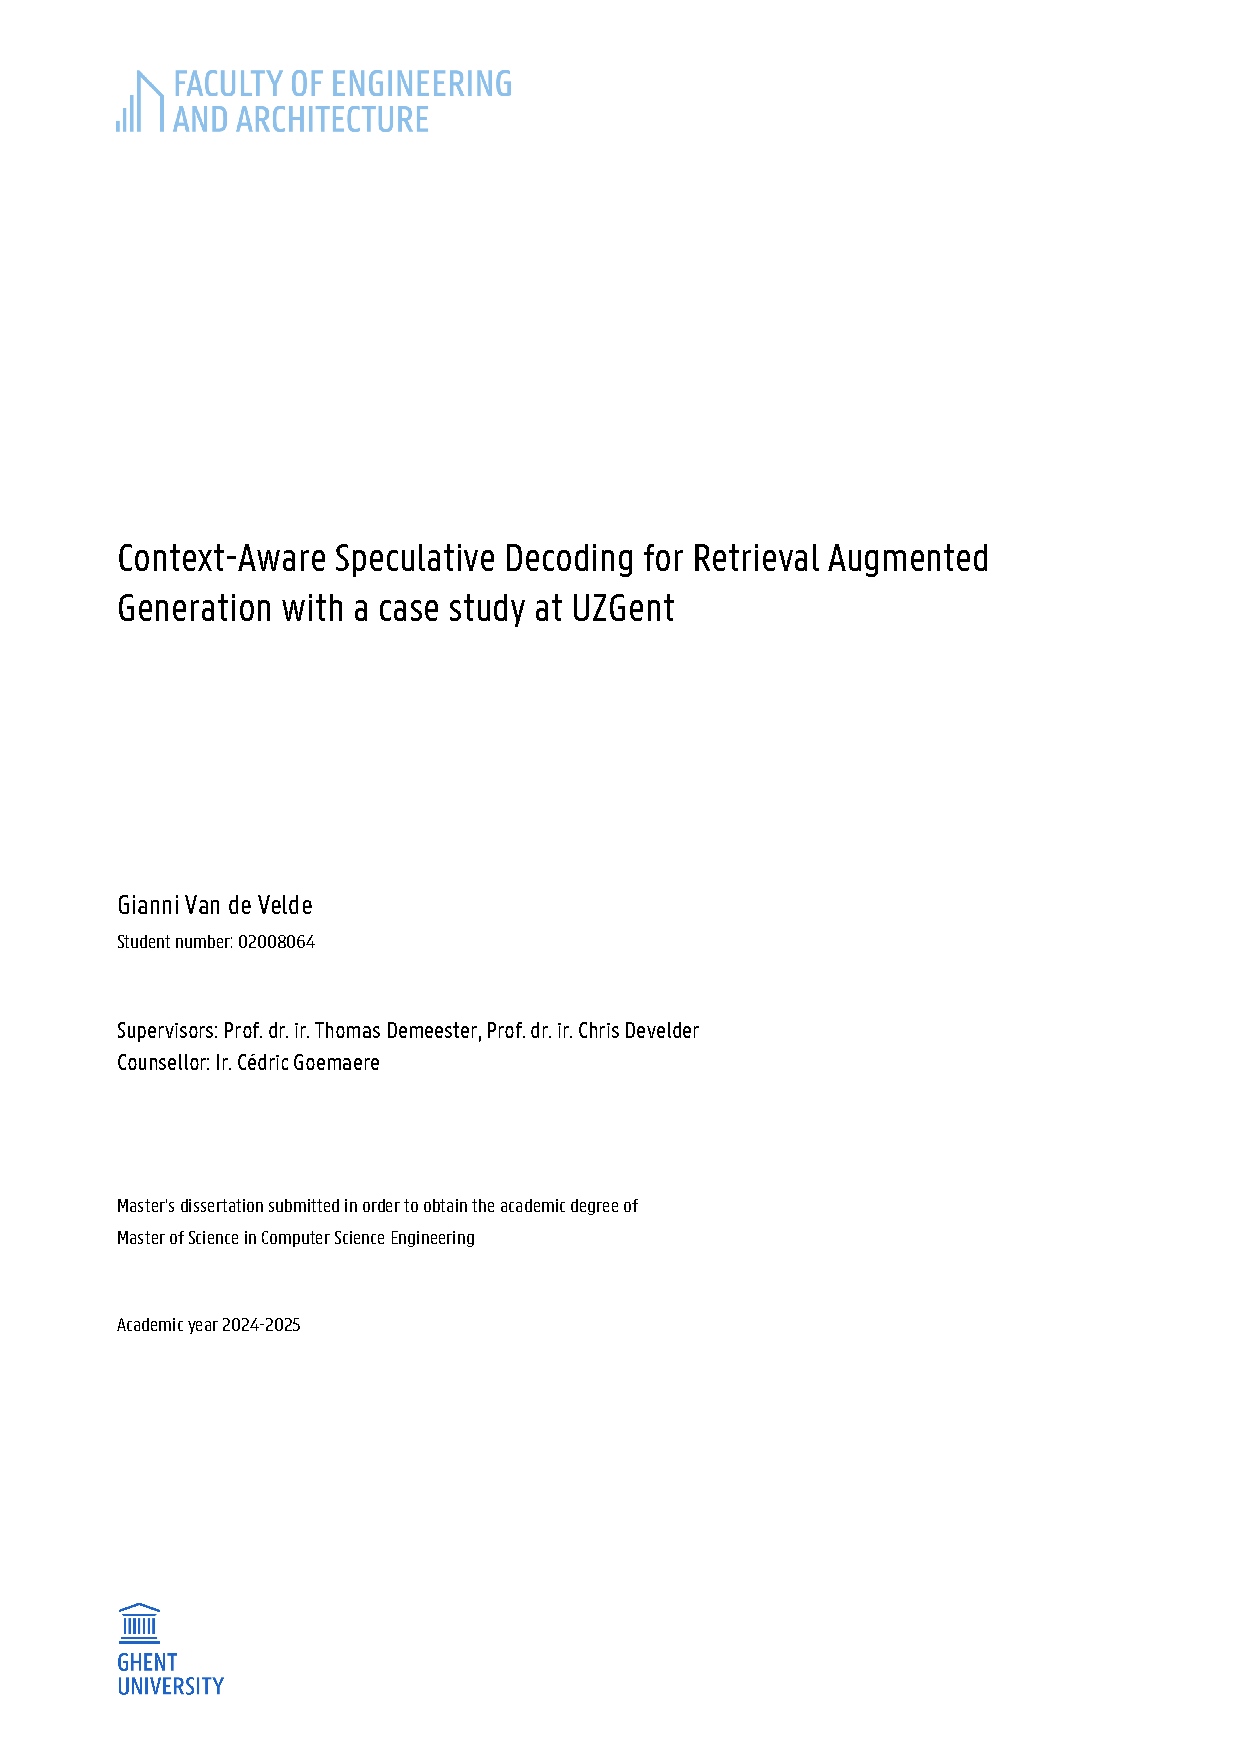
\includepdf{titlepage/titlepage.pdf}

    \newpage
    \newpage
    
    \titleformat{\chapter}{}{}{0em}{\bf\Huge}

    \afterpage{\blankpage}

    \pagenumbering{roman}

    \import{additional-sections/preface/}{content.tex}
    \import{additional-sections/permissionofloan/}{content.tex}
    \import{additional-sections/explanatorynote}{content.tex}
    \import{additional-sections/abstract/}{content.tex}
    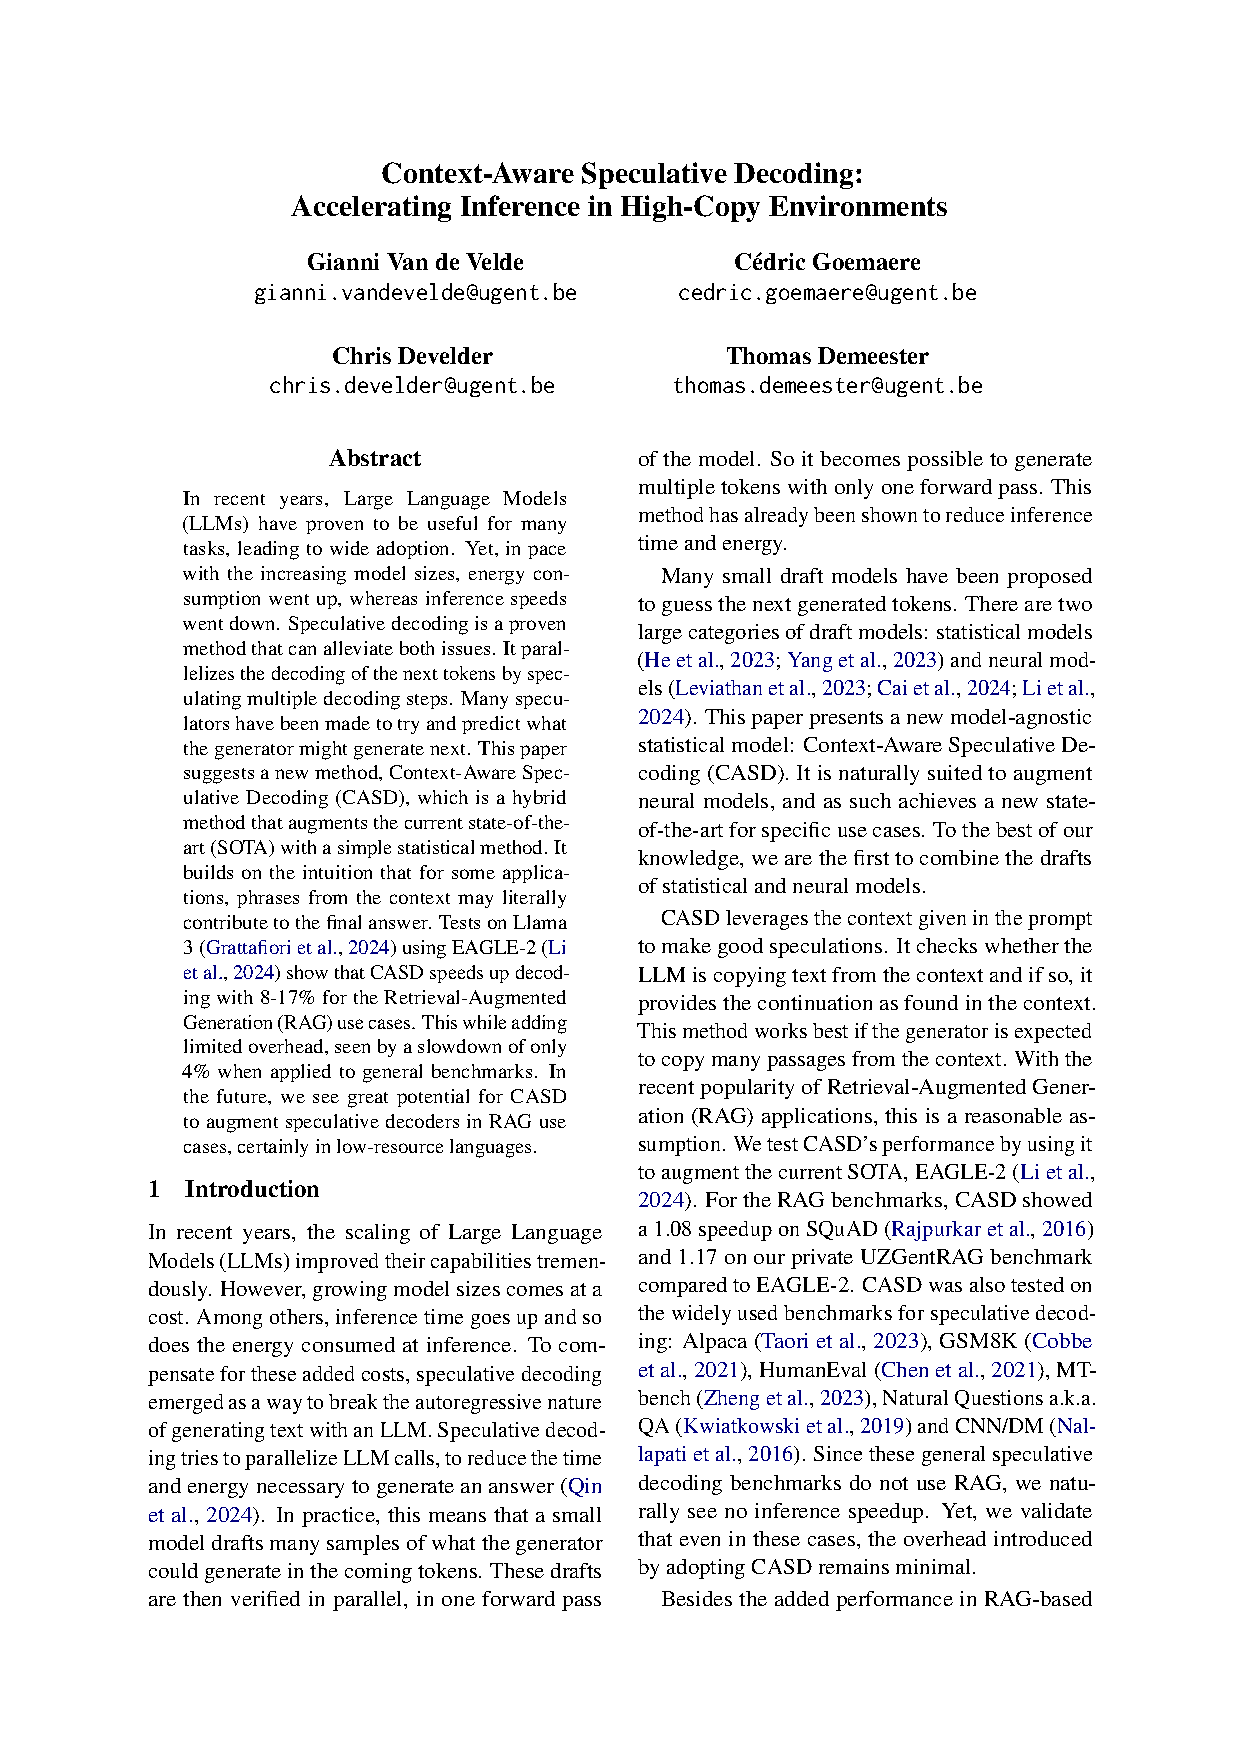
\includepdf[pages={1-}]{extendedabstract/extended-abstract.pdf}

    \tableofcontents

    % table of figures / table of tables

    % list of acronyms
    
    \titleformat{\chapter}[display]{\normalfont\bfseries\Huge}{\chaptertitlename\ \thechapter}{1em}{\bf\Huge}

    \newpage
    \pagenumbering{arabic}

    \import{chapters/introduction/}{content.tex}
    \import{chapters/rag/}{content.tex}
    \import{chapters/usecase_UZ/}{content.tex}
    \import{chapters/speculative_decoding/}{content.tex}
    \import{chapters/context_aware_speculative_decoding/}{content.tex}
    % add chapters here

    % society impact
    \import{chapters/societalimpact/}{content.tex}

    \import{chapters/conclusions_and_future_work/}{content.tex}

    \printbibliography
    \addcontentsline{toc}{chapter}{Bibliography}

    \appendix
    \import{appendices/example/}{content.tex}

    \afterpage{\blankpage}

    % \makeback
\end{document}